\جزوحصہء{سوالات}
\موٹا{یک رتبی جزوی تفرق کی تلاش}\\
سوال \حوالہ{ سوال_کثیرالمتغیر_یک_رتبی_جزوی_الف}  تا سوال  \حوالہ{سوال_کثیرالمتغیر_یک_رتبی_جزوی_ب} میں \عددی{\tfrac{\partial f}{\partial x}} اور \عددی{\tfrac{\partial f}{\partial y}} تلاش کریں۔

\ابتدا{سوال}\شناخت{ سوال_کثیرالمتغیر_یک_رتبی_جزوی_الف}
$f(x,y)=2x^2-3y-4$
\انتہا{سوال}
%===================
\ابتدا{سوال}
$f(x,y)=x^2-xy+y^2$
\انتہا{سوال}
%====================
\ابتدا{سوال}
$f(x,y)=(x^2-1)(y+2)$
\انتہا{سوال}
%====================
\ابتدا{سوال}
$f(x,y)=5xy-7x^2-y^2+3x-6y+2$
\انتہا{سوال}
%====================
\ابتدا{سوال}
$f(x,y)=(xy-1)^2$
\انتہا{سوال}
%====================
\ابتدا{سوال}
$f(x,y)=(2x-3y)^3$
\انتہا{سوال}
%====================
\ابتدا{سوال}
$f(x,y)=\sqrt{x^2+y^2}$
\انتہا{سوال}
%====================
\ابتدا{سوال}
$f(x,y)=(x^3+y/2)^{2/3}$
\انتہا{سوال}
%====================
\ابتدا{سوال}
$f(x,y)=\frac{1}{x+y}$
\انتہا{سوال}
%====================
\ابتدا{سوال}
$f(x,y)=\frac{x}{x^2+y^2}$
\انتہا{سوال}
%====================
\ابتدا{سوال}
$f(x,y)=\frac{x+y}{xy-1}$
\انتہا{سوال}
%====================
\ابتدا{سوال}
$f(x,y)=\tan^{-1}\frac{y}{x}$
\انتہا{سوال}
%====================
\ابتدا{سوال}
$f(x,y)=e^{x+y+1}$
\انتہا{سوال}
%====================
\ابتدا{سوال}
$f(x,y)=e^{-x}\sin(x+y)$
\انتہا{سوال}
%====================
\ابتدا{سوال}
$f(x,y)=\ln(x+y)$
\انتہا{سوال}
%====================
\ابتدا{سوال}
$f(x,y)=e^{xy}\ln y$
\انتہا{سوال}
%====================
\ابتدا{سوال}
$f(x,y)=\sin^2(x-3y)$
\انتہا{سوال}
%====================
\ابتدا{سوال}
$f(x,y)=\cos^2(3x-y^2)$
\انتہا{سوال}
%====================
\ابتدا{سوال}
$f(x,y)=x^y$
\انتہا{سوال}
%====================
\ابتدا{سوال}
$f(x,y)=\log_y x$
\انتہا{سوال}
%====================
\ابتدا{سوال}
$f(x,y)=\int_x^yg(t)\dif t\quad \text{\RL{تمام \عددی{t} کے لئے \عددی{g} استمراری ہے}}$
\انتہا{سوال}
%====================
\ابتدا{سوال}\شناخت{سوال_کثیرالمتغیر_یک_رتبی_جزوی_ب}
$f(x,y)=\sum\limits_{n=0}^{\infty}(xy)^n\quad (\abs{xy}<1)$
\انتہا{سوال}
%====================

سوال \حوالہ{سوال_کثیرالمتغیر_یک_رتبی_تین_متغیر_تفاعل_الف} تا سوال \حوالہ{سوال_کثیرالمتغیر_یک_رتبی_تین_متغیر_تفاعل_ب} میں \عددی{f_x}، \عددی{f_y}  اور \عددی{f_z} تلاش کریں۔

\ابتدا{سوال}\شناخت{سوال_کثیرالمتغیر_یک_رتبی_تین_متغیر_تفاعل_الف}
$f(x,y,z)=1+xy^2-2z^2$
\انتہا{سوال}
%===================
\ابتدا{سوال}
$f(z,y,z)=xy+yz+xz$
\انتہا{سوال}
%=====================
\ابتدا{سوال}
$f(z,y,z)=x-\sqrt{y^2+z^2}$
\انتہا{سوال}
%=====================
\ابتدا{سوال}
$f(z,y,z)=(x^2+y^2+z^2)^{-1/2}$
\انتہا{سوال}
%=====================
\ابتدا{سوال}
$f(z,y,z)=\sin^{-1}(xyz)$
\انتہا{سوال}
%=====================
\ابتدا{سوال}
$f(z,y,z)=\sec^{-1}(x+yz)$
\انتہا{سوال}
%=====================
\ابتدا{سوال}
$f(z,y,z)=\ln(x+2y+3z)$
\انتہا{سوال}
%=====================
\ابتدا{سوال}
$f(z,y,z)=yz\ln(xy)$
\انتہا{سوال}
%=====================
\ابتدا{سوال}
$f(z,y,z)=e^{-(x^2+y^2+z^2)}$
\انتہا{سوال}
%=====================
\ابتدا{سوال}
$f(z,y,z)=e^{-xyz}$
\انتہا{سوال}
%=====================
\ابتدا{سوال}
$f(z,y,z)=\tanh(x+2y+3z)$
\انتہا{سوال}
%=====================
\ابتدا{سوال}\شناخت{سوال_کثیرالمتغیر_یک_رتبی_تین_متغیر_تفاعل_ب}
$f(z,y,z)=\sinh(xy-z^2)$
\انتہا{سوال}
%=====================

سوال \حوالہ{سوال_کثیر_المتغیر_ہر_متغیر_جزوی_الف} تا سوال \حوالہ{سوال_کثیر_المتغیر_ہر_متغیر_جزوی_ب} میں ہر متغیر کے لحاظ سے تفاعل کا جزوی تفرق تلاش کریں۔

\ابتدا{سوال}\شناخت{سوال_کثیر_المتغیر_ہر_متغیر_جزوی_الف}
$f(t,\alpha)=\cos(2\pi t-\alpha)$
\انتہا{سوال}
%=================
\ابتدا{سوال}
$g(u,v)=v^2e^{2u/v}$
\انتہا{سوال}
%=================
\ابتدا{سوال}
$h(\rho,\phi,\theta)=\rho\sin\phi\cos\theta$
\انتہا{سوال}
%=================
\ابتدا{سوال}
$g(r,\theta,z)=r(1-\cos\theta)-z$
\انتہا{سوال}
%=================
\ابتدا{سوال}\ترچھا{قلب کا کام}\\
$W(P,H,\delta,v,g)=PV+\frac{H\delta v^2}{2g}$
\انتہا{سوال}
%=================
\ابتدا{سوال}\شناخت{سوال_کثیر_المتغیر_ہر_متغیر_جزوی_ب}
$A(c,h,k,m,q)=\frac{km}{q}+cm+\frac{hq}{2}$
\انتہا{سوال}
%=================

\موٹا{دو رتبی جزوی تفرق کا حصول}\\
سوال \حوالہ{سوال_کثیرالمتغیر_تمام_جزوی_تلاش_الف} تا سوال \حوالہ{سوال_کثیرالمتغیر_تمام_جزوی_تلاش_ب} میں تفاعل کے تمام دو رتبی جزوی تفرقات تلاش کریں۔

\ابتدا{سوال}\شناخت{سوال_کثیرالمتغیر_تمام_جزوی_تلاش_الف}
$f(x,y)=x+y+xy$
\انتہا{سوال}
%=================
\ابتدا{سوال}
$f(x,y)=\sin xy$
\انتہا{سوال}
%=================
\ابتدا{سوال}
$g(x,y)=x^2y+\cos y+y\sin x$
\انتہا{سوال}
%=================
\ابتدا{سوال}
$h(x,y)=xe^y+y+1$
\انتہا{سوال}
%=================
\ابتدا{سوال}
$r(x,y)=\ln(x,y)$
\انتہا{سوال}
%=================
\ابتدا{سوال}\شناخت{سوال_کثیرالمتغیر_تمام_جزوی_تلاش_ب}
$s(x,y)=\tan^{-1}\frac{y}{x}$
\انتہا{سوال}
%=================

\موٹا{مدغم جزوی تفرقات}\\
سوال \حوالہ{سوال_کثیرالمتغیر_تصدیق_مدغم_الف} تا سوال \حوالہ{سوال_کثیرالمتغیر_تصدیق_مدغم_ب}   میں \عددی{w_{xy}=w_{yx}} کی   تصدیق کریں۔

\ابتدا{سوال}\شناخت{سوال_کثیرالمتغیر_تصدیق_مدغم_الف}
$w=\ln(2x+3y)$
\انتہا{سوال}
%===============
\ابتدا{سوال}
$w=e^x+x\ln y+y]ln x$
\انتہا{سوال}
%==================
\ابتدا{سوال}
$w=xy^2+x^2y^3+x^3y^4$
\انتہا{سوال}
%==================
\ابتدا{سوال}\شناخت{سوال_کثیرالمتغیر_تصدیق_مدغم_ب}
$w=x\sin y+y\sin x+xy$
\انتہا{سوال}
%==================
\ابتدا{سوال}
بغیر قلم اٹھائے   بتائیں کہ درج ذیل میں \عددی{x} کے لحاظ سے پہلے اور \عددی{y} کے  لحاظ سے بعد میں یا اس کے الٹ حل کرتے ہوئے  \عددی{f_{xy}} زیادہ جلدی حاصل ہو گا۔
\begin{enumerate}[a.]
\item
$f(x,y)=x\sin y+e^y$
\item
$f(x,y)=\frac{1}{x}$
\item
$f(x,y)=y+\frac{x}{y}$
\item
$f(x,y)=y+x^2y+4y^3-\ln(y^2+1)$
\item
$f(x,y)=x^2+5xy+\sin x+7e^x$
\item
$f(x,y)=x\ln xy$
\end{enumerate}
\انتہا{سوال}
%===============
\ابتدا{سوال}
درج ذیل میں تمام کا پانچ رتبی جزوی تفرق \عددی{\tfrac{\partial^{\,5}f}{\partial x^2\partial y^3}} صفر کے برابر ہے۔ اس کی تصدیق کرنے کی خاطر آپ کس متغیر کے لحاظ سے پہلے جزوی تفرق لیں گے؟ بغیر کچھ لکھے جواب دینے کی کوشش کریں۔
\begin{enumerate}[a.]
\item
$f(x,y)=y^2x^4e^x+2$
\item
$f(x,y)=y^2+y(\sin x-x^4)$
\item
$f(x,y)=x^2+5xy+\sin x+7e^x$
\item
$f(x,y)=xe^{y^2/2}$
\end{enumerate}
\انتہا{سوال}
%==============

\موٹا{جزوی تفرق کی تعریف کا استعمال}\\
سوال \حوالہ{سوال_کثیرالمتغیر_تعریف_حد_جزوی_تفرق_الف} اور سوال \حوالہ{سوال_کثیرالمتغیر_تعریف_حد_جزوی_تفرق_ب} میں جزوی تفرق کی تعریف بذریعہ حد استعمال کرتے ہوئے دیے گئے نقطہ پر تفاعل کا جزوی تفرق حاصل کریں۔

\ابتدا{سوال}\شناخت{سوال_کثیرالمتغیر_تعریف_حد_جزوی_تفرق_الف}
$f(x,y)=1-x+y-3x^2y,\quad \frac{\partial f}{\partial x},\,\frac{\partial f}{\partial y},\quad (1,2)$
\انتہا{سوال}
%==================
\ابتدا{سوال}\شناخت{سوال_کثیرالمتغیر_تعریف_حد_جزوی_تفرق_ب}
$f(x,y)=4+2x-3y-xy^2,\quad \frac{\partial f}{\partial x},\,\frac{\partial f}{\partial y},\quad (-2,1)$
\انتہا{سوال}
%=================
\ابتدا{سوال}
فرض کریں \عددی{w=f(x,y,z)} تین غیر تابع متغیرات کا تفاعل ہے۔ نقطہ \عددی{(x_0,y_0,z_0)} پر جزوی تفرق  \عددی{\tfrac{\partial f}{\partial z}} کی باضابطہ تعریف  لکھیں کریں۔ اس تعریف کو استعمال کرتے ہوئے \عددی{(1,2,3)} پر \عددی{f(x,y,z)=x^2yz^2} کا \عددی{\tfrac{\partial f}{\partial z}} تلاش کریں۔
\انتہا{سوال}
%===================
\ابتدا{سوال}
فرض کریں \عددی{w=f(x,y,z)} تین غیر تابع متغیرات کا تفاعل ہے۔ نقطہ \عددی{(x_0,y_0,z_0)} پر جزوی تفرق  \عددی{\tfrac{\partial f}{\partial y}} کی باضابطہ تعریف  لکھیں کریں۔ اس تعریف کو استعمال کرتے ہوئے \عددی{(-1,0,3)} پر \عددی{f(x,y,z)=-2xy^2+yz^2} کا \عددی{\tfrac{\partial f}{\partial z}} تلاش کریں۔
\انتہا{سوال}
%===============
\موٹا{خفی جزوی تفرقات}\\
\ابتدا{سوال}
 ذیل مساوات  میں     غیر تابع متغیرات \عددی{x} اور \عددی{y} کا تفاعل \عددی{z} پیش کیا گیا ہے۔ نقطہ \عددی{(1,1,1)} پر \عددی{\tfrac{\partial z}{\partial x}} کی قیمت تلاش کریں۔ اس نقطہ پر   یہ  جزوی تفرق  موجود ہے۔  
\begin{align*}
xy+z^3x-2yz=0
\end{align*}
\انتہا{سوال}
%====================
\ابتدا{سوال}
 ذیل مساوات  میں     غیر تابع متغیرات \عددی{x} اور \عددی{y} کا تفاعل \عددی{z} پیش کیا گیا ہے۔ نقطہ \عددی{(1,-1,-3)} پر \عددی{\tfrac{\partial z}{\partial x}} کی قیمت تلاش کریں۔ اس نقطہ پر   یہ  جزوی تفرق  موجود ہے۔  
\begin{align*}
xz+y\ln x-x^2+4=0
\end{align*}
\انتہا{سوال}
%===================
سوال \حوالہ{سوال_کثیرالمتغیر_مثلث_الف} اور سوال \حوالہ{سوال_کثیرالمتغیر_مثلث_الف} درج ذیل مثلث  کے بارے میں ہے۔
\begin{center}
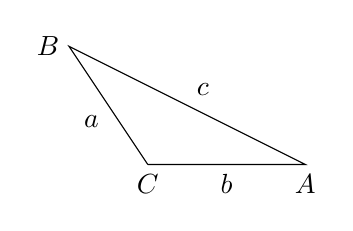
\begin{tikzpicture}
\draw(0,0)node[below]{$C$}--(2,0)node[below]{$A$}node[pos=0.5,below]{$b$}--(-1,1.5)node[left]{$B$}node[pos=0.5,above right]{$c$}--(0,0)node[pos=0.5,below left]{$a$};
\end{tikzpicture}
\end{center}

\ابتدا{سوال}\شناخت{سوال_کثیرالمتغیر_مثلث_الف}
\عددی{A} کو خفی طور پر \عددی{a}، \عددی{b} اور \عددی{c} کا تفاعل لکھ کر \عددی{\tfrac{\partial A}{\partial a}} اور \عددی{\tfrac{\partial A}{\partial b}} تلاش کریں۔
\انتہا{سوال}
%=================
\ابتدا{سوال}\شناخت{سوال_کثیرالمتغیر_مثلث_ب}
\عددی{a} کو خفی طور پر \عددی{A}، \عددی{b} اور \عددی{B} کا تفاعل لکھ کر \عددی{\tfrac{\partial a}{\partial A}} اور \عددی{\tfrac{\partial a}{\partial B}} تلاش کریں۔
\انتہا{سوال}
%=================
\ابتدا{سوال}\شناخت{سوال_کثیرالمتغیر_پیچیدہ_مساوات}
غیر تابع متغیرات \عددی{x} اور \عددی{y} کی صورت میں تفاعل  \عددی{u} اور \عددی{v} مساوات \عددی{x=v\ln u} اور \عددی{y=u\ln v} دیتی ہیں۔ جزوی تفرق \عددی{v_x} ،  جو موجود ہے، کو \عددی{u} اور \عددی{v} کی صورت میں لکھیں۔ (اشارہ: دونوں مساوات کا تفرق  \عددی{x} ا کے لحاظ سے لے کر \عددی{v_x} کے لئے حل کریں۔)
\انتہا{سوال}
%=====================
\ابتدا{سوال}
غیر تابع متغیرات \عددی{u} اور \عددی{v} کی صورت میں تفاعل  \عددی{x} اور \عددی{y} مساوات \عددی{u=x^2-y^2} اور \عددی{v=x^2-y} دیتی ہیں۔ جزوی تفرق \عددی{\tfrac{\partial x}{\partial u}} اور  \عددی{\tfrac{\partial y}{\partial u}} ،  جو موجود  ہیں تلاش کریں۔ (اشارہ:سوال \حوالہ{سوال_کثیرالمتغیر_پیچیدہ_مساوات} میں دیا گیا اشارہ دیکھیں۔)   اس کے بعد \عددی{s=x^2+y} لیتے ہوئے \عددی{\tfrac{\partial s}{\partial u}} حاصل کریں۔
\انتہا{سوال}
%=====================
\موٹا{مساوات لاپلاس}\\
\ترچھا{تین بعدی مساوات لاپلاس}
\begin{align}\label{مساوات_کثیر_المتغیر_مساوات_لاپلاس_الف}
\frac{\partial^{\,2}f}{\partial x^2}+\frac{\partial^{\,2}f}{\partial y^2}+\frac{\partial^{\,2}f}{\partial z^2}=0
\end{align}
کو فضا میں  برقرار حال حراری تقسیم \عددی{T=f(x,y,z)}، تجاذبی  مخفی قوہ اور برقی ساکن مخفی قوہ   مطمئن کرتے ہیں۔ مساوات \حوالہ{مساوات_کثیر_المتغیر_مساوات_لاپلاس_الف} سے جزو \عددی{\tfrac{\partial f}{\partial z}} نکالنے سے    \ترچھا{دو بعدی مساوات لاپلاس}
 \begin{align}\label{مساوات_کثیر_المتغیر_مساوات_لاپلاس_ب}
\frac{\partial^{\,2}f}{\partial x^2}+\frac{\partial^{\,2}f}{\partial y^2}=0
\end{align}
حاصل ہوتی ہے جو مستوی میں  خفی قوہ اور برقرار حال حراری تقسیم  بیان کرتی ہے۔

دکھائیں کہ سوال \حوالہ{سوال_کثیرالمتغیر_مطمئن_لاپلاس_الف} تا سوال \حوالہ{سوال_کثیرالمتغیر_مطمئن_لاپلاس_ب} میں  دیا ہر ایک  تفاعل مساوات لاپلاس میں سے کسی ایک کو مطمئن کرتا ہے۔ 

\ابتدا{سوال}\شناخت{سوال_کثیرالمتغیر_مطمئن_لاپلاس_الف}
$f(x,y,z)=x^2+y^2-2z^2$
\انتہا{سوال}
%==============
\ابتدا{سوال}
$f(x,y,z)=2z^3-3(x^2+y^2)z$
\انتہا{سوال}
%=====================
\ابتدا{سوال}
$f(x,y)=e^{-2y}\cos 2x$
\انتہا{سوال}
%=====================
\ابتدا{سوال}
$f(x,y)=\ln\sqrt{x^2+y^2}$
\انتہا{سوال}
%=====================
\ابتدا{سوال}
$f(x,y,z)=(x^2+y^2+z^2)^{-1/2}$
\انتہا{سوال}
%=====================
\ابتدا{سوال}\شناخت{سوال_کثیرالمتغیر_مطمئن_لاپلاس_ب}
$f(x,y,z)=e^{2x+4y}\cos 5z$
\انتہا{سوال}
%=====================

\موٹا{مساوات موج}\\
سمندر  کے کنارے کھڑے  ہو کر سمندری امواج کی لی گئی  تصویر  میں نشیب و فراز کا   ایک منظم نقش نظر آتا ہے۔ہمیں  فضا میں  فاصلہ کے لحاظ سے   دوری انتصابی حرکت نظر آتی ہے۔ پانی میں کھڑے ہو کر ہم گزرتی امواج کی بنا پانی کا اتار چھڑاو محسوس کرتے ہیں۔ ہم وقت کے لحاظ سے دوری انتصابی حرکت  دیکھتے ہیں۔طبیعیات  میں اس خوبصورت   تشاکلی کو \ترچھا{یک بعدی مساوات موج}
\begin{align}
\frac{\partial^{\,2}u}{\partial t^2}=c^2\frac{\partial ^{\,2}w}{\partial x^2}
\end{align}
بیان کرتی ہے جہاں  قد موج  \عددی{w}، فاصلاتی متغیر  \عددی{x}، لمحاتی متغیر \عددی{t} اور موج کی رفتار  \عددی{c}  ہے۔ 

سمندری سطح پر فاصلہ \عددی{x} ہو گا لیکن دیگر عملی استعمال میں \عددی{x}  ارتعاش پذیر  تار کے ساتھ ساتھ  فاصلہ، ہوا میں فاصلہ (صوتی امواج)، یا فضا میں فاصلہ  (امواج نور)  ہو سکتا ہے۔  عدد \عددی{c} کی قیمت موج کی قسم اور  ذریعہ پر منحصر ہو  گا۔

دکھائیں کہ سوال \حوالہ{سوال_کثیرالمتغیر_مساوات_موج_الف} تا سوال \حوالہ{سوال_کثیرالمتغیر_مساوات_موج_ب}  میں تمام  تفاعل مساوات موج کو مطمئن کرتے ہیں۔ 

\ابتدا{سوال}\شناخت{سوال_کثیرالمتغیر_مساوات_موج_الف}
$w=\sin(x+ct)$
\انتہا{سوال}
%===================
\ابتدا{سوال}
$w=\cos(2x+2ct)$
\انتہا{سوال}
%==================
\ابتدا{سوال}
$w=\sin(x+ct)+\cos(2x+2ct)$
\انتہا{سوال}
%==================
\ابتدا{سوال}
$w=\ln(2x+2ct)$
\انتہا{سوال}
%==================
\ابتدا{سوال}
$w=\tan(2x-2ct)$
\انتہا{سوال}
%==================
\ابتدا{سوال}
$w=5\cos(3x+3ct)+e^{x+ct}$
\انتہا{سوال}
%==================
\ابتدا{سوال}\شناخت{سوال_کثیرالمتغیر_مساوات_موج_ب}
$w=f(u)$
جہاں \عددی{f} متغیر \عددی{u} کا قابل تفرق تفاعل ہے اور \عددی{u=a(x+ct)} ہے جس میں \عددی{a} مستقل ہے۔
\انتہا{سوال}
%==================
